\section{Feladat}

\subsection{Cél}
Egy csomag mozgatása egy gyári környezetben, a szintkülönbség áthídalásához a csomag felemelése és tovább tolása.
\begin{figure}[!hbt]
    \centering
    \includegraphics[width=0.5\textwidth]{res/imgs/drawing.jpg}
    \caption{Grafikus szimuláció}
    \label{fig:drawing}
\end{figure}

\newpage
\subsection{Megoldás}
A feladatban egy csomag mozgatását oldjuk meg szállítószalaggon.
A csomag az alsó szállítószalagon jön be, ahol szenzor figyeli a csomag jelenlétét.
Amint a csomag megérkezik az alsó munkahenger kitolja ezzel felemelve.
Szenzor figyeli az alsó munkahengert, melynek hatására a rendszer kitolja a felső munkahengert ezzel továbbítva a csomagot ami kiugrik a munkaterületről.
A végén a munkahengerek visszatérnek alaphelyzetükbe.
\begin{figure}[!hbt]
    \centering
    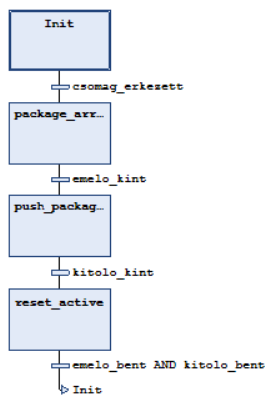
\includegraphics[width=0.5\textwidth]{res/imgs/PLC_PRG_sfc.png}
    \caption{Vezérlő logika SFC}
    \label{fig:sfc_logic}
\end{figure}

\newpage
\section{Megvalósítás}
\begin{figure}[!hbt]
    \centering
    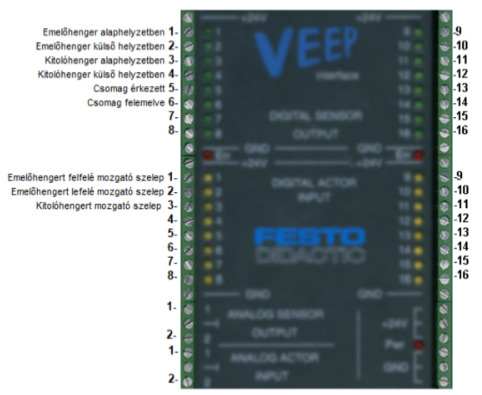
\includegraphics[width=0.7\textwidth]{res/imgs/veep_io.png}
    \caption{VEEP interface lábkiosztás}
    \label{fig:veep_io}
\end{figure}

\begin{figure}[!hbt]
    \centering
    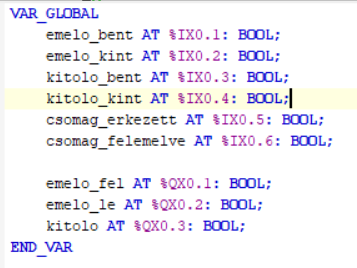
\includegraphics[width=0.6\textwidth]{res/imgs/GVL.png}
    \caption{Globális változók deklarálása (GVL)}
    \label{fig:gvl}
\end{figure}

\newpage
A fő vezérlés SFC-ben íródott, az állapotokat pedig LD-ben valósítottuk meg.

A csomag érkezésekor a függőleges munkahengert kitoljuk. (Mivel két bemenettel lehet vezérelni, az ellentétes állapotot negáljuk.)
\begin{figure}[!hbt]
    \centering
    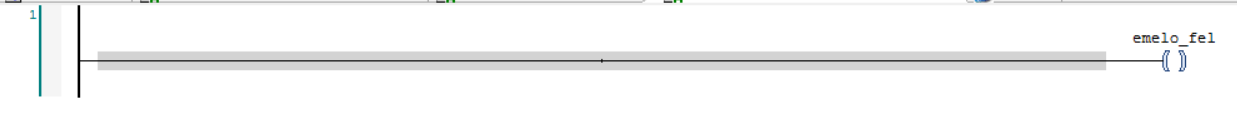
\includegraphics[width=0.9\textwidth]{res/imgs/package_arrived_ld.png}
    \caption{Csomag érkezését kezelő létra diagram (package\_arrived)}
    \label{fig:ld_arrived}
\end{figure}

Amint felér a csomag, a vízszintes munkahengerrel kitoljuk a szállítószalagra.
\begin{figure}[!hbt]
    \centering
    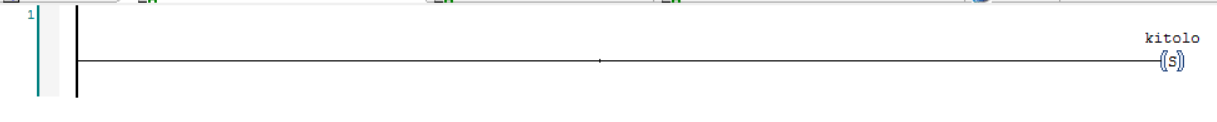
\includegraphics[width=0.9\textwidth]{res/imgs/push_package_active_ld.png}
    \caption{Csomag kitolását végző létra diagram (push\_package\_active)}
    \label{fig:ld_push}
\end{figure}

A csomag továbbítása után alaphelyzetbe állítjuk a rendszert. (Tehát a két munkahengert visszahúzzuk.)
\begin{figure}[!hbt]
    \centering
    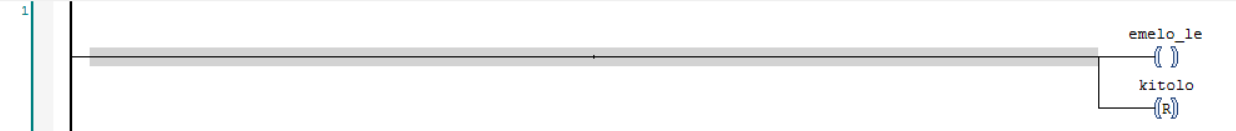
\includegraphics[width=0.9\textwidth]{res/imgs/reset_active_ld.png}
    \caption{Alaphelyzetbe állást végző létra diagram (reset\_active)}
    \label{fig:ld_reset}
\end{figure}